\chapter{Stato dell'arte}
\label{sec:3_stato_arte}

In questo capitolo sono riportati alcuni studi presenti nella letteratura scientifica relativi alla distribuzione del lavoro in ambienti edge ed edge-cloud, considerando sia approcci euristici \cite{Chai2021, Hsieh2023} sia basati sull'Apprendimento per Rinforzo \cite{Liu2023, Zhang2023}. In questo contesto, il machine learning e in particolare il RL hanno recentemente acquisito popolarità, per via della loro capacità di effettuare decisioni rapide sulla distribuzione del lavoro in ambienti dinamici e parzialmente osservabili \cite{Hortelano2023, Kar2023}.

\section{Survey su approcci basati su ML/RL}

In \cite{Kar2023} viene presentato un ampio sondaggio sui metodi di ottimizzazione proposti in letteratura per la distribuzione del lavoro in ambienti federati che utilizzano più paradigmi di computazione. Viene proposta una classificazione degli ambienti, in base ai paradigmi utilizzati e la tipologia di federazione (orizzontale o verticale). Vengono inoltre definiti i possibili metodi di distribuzione del lavoro (es. da edge a edge o da edge a cloud) e gli scenari, mostrati in \Cref{fig:2_task_offloading_scenarios}: il primo scenario (1) coinvolge dispositivi in una posizione localizzata con poca mobilità, il secondo (2) coinvolge i veicoli con grande mobilità, mentre il terzo (3) descrive il traffico generato dai dispositivi IoT industriali. Ogni scenario ha le sue caratteristiche e richieste in termini di latenza e qualità del servizio.

\begin{figure}
    \centering
    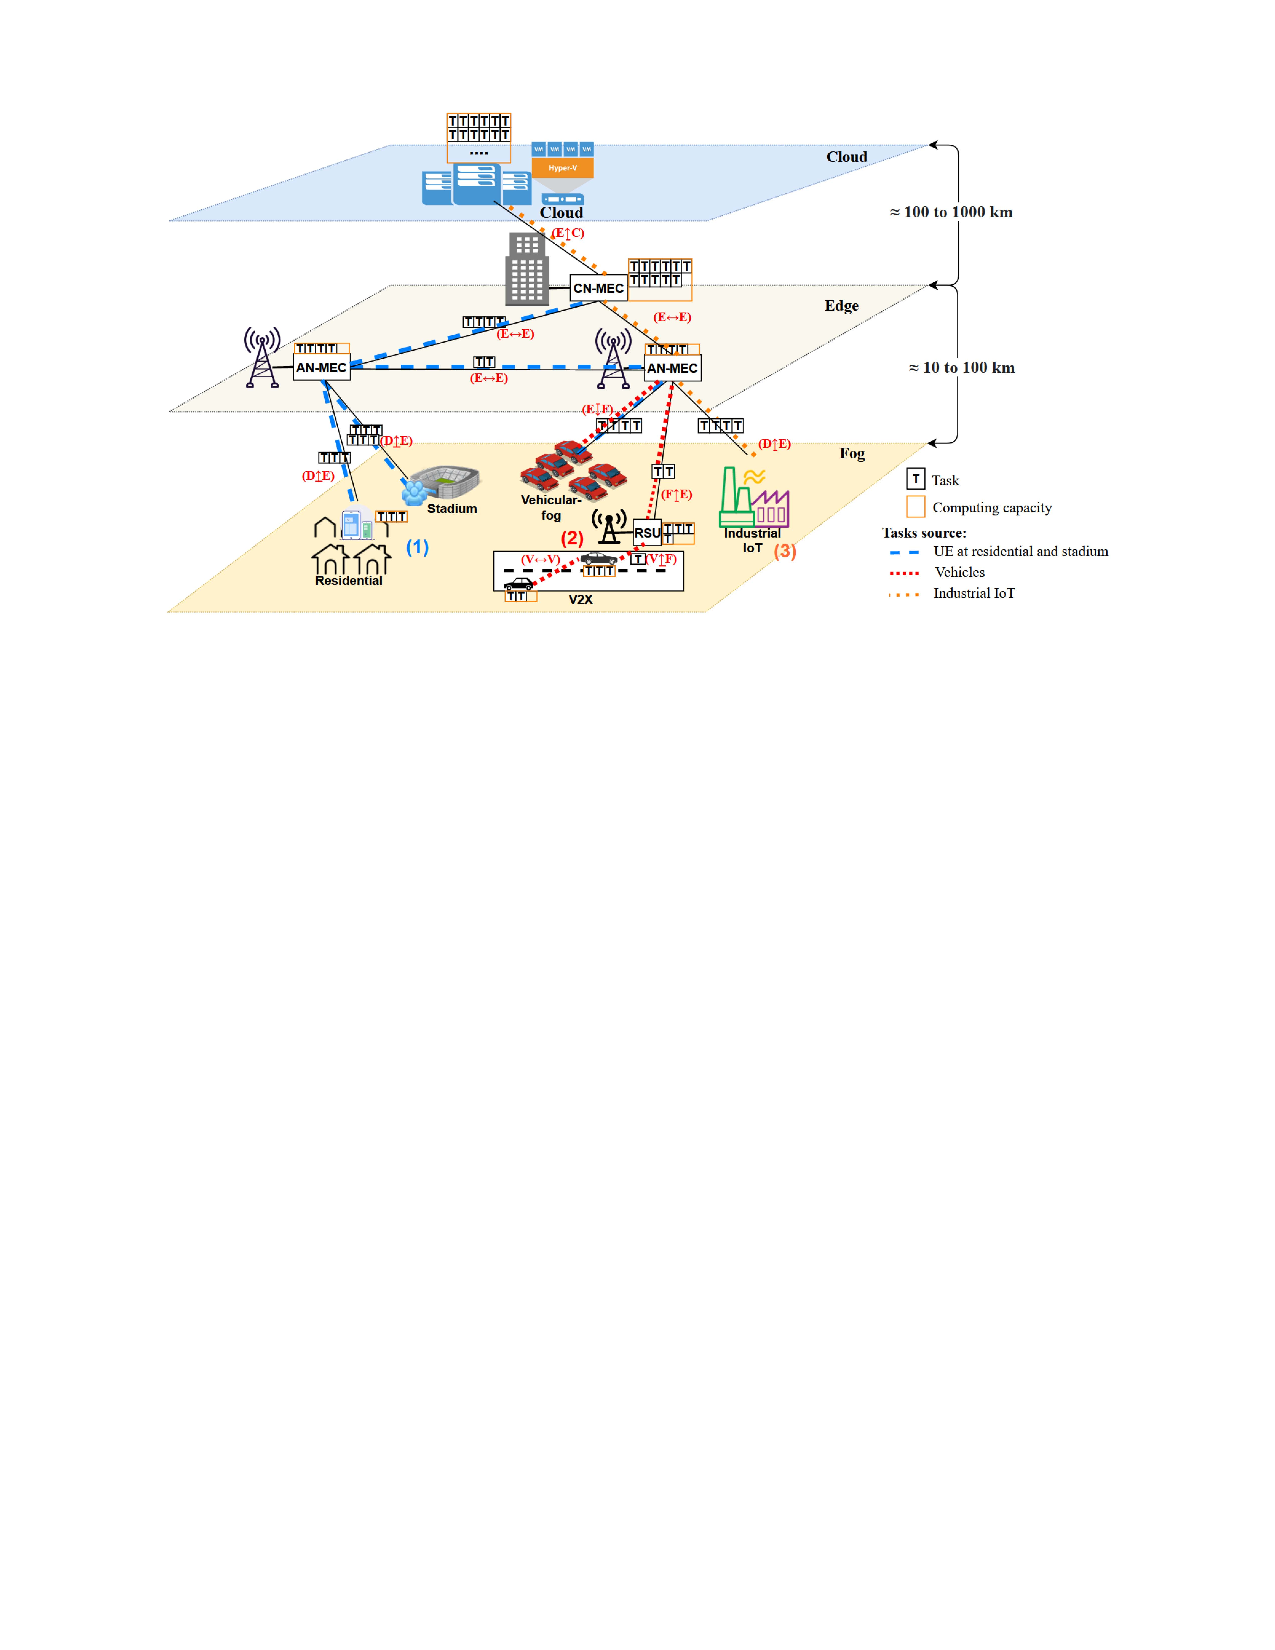
\includegraphics[width=\textwidth]{assets/3/task_offloading_scenarios.pdf}
    \caption[Distribuzione del lavoro nel cloud-edge-fog federato]{Distribuzione del lavoro nel cloud-edge-fog federato. Fonte: \cite{Kar2023}}
    \label{fig:2_task_offloading_scenarios}
\end{figure}

In base alla tipologia di ambiente e di scenario sono presentati una serie di approcci, partendo dai metodi di ottimizzazione tradizionali, che svolgono una ricerca spesso esaustiva per trovare una soluzione ottimale e richiedono una conoscenza esatta del sistema. Tra i lavori presentati, la maggior parte fanno uso di euristiche (metodo di bisezione, ottimizzazione iterativa a due fasi) oppure di algoritmi dinamici, valutati principalmente su ambienti simulati e che si concentrano sulla gestione del traffico. Metodi di questo tipo richiedono troppo tempo per convergere in scenari di larga scala e che devono garantire una latenza ridotta. Per questo approcci, di tipo ML hanno acquisito popolarità, in particolare il Deep Learning. Un limite dell'apprendimento supervisionato, tuttavia, è la necessità di richiedere un insieme di dati etichettato, non sempre possibile in ambienti così dinamici come può essere la rete, oltre a essere poco adattabile in nuovi scenari incontrati. Il RL, invece, ha ottime proprietà di adattamento poiché apprende tramite l'interazione diretta con l'ambiente. Tra i vari studi presentati che usano il RL e il Deep RL, la maggior parte adotta gli algoritmi DPPG\footnote{Deep Deterministic Policy Gradient.} e DQN\footnote{Deep Q-Network.}, entrambi di tipo off-policy e addestrati su ambienti simulati e per applicazioni relative ai tre scenari individuati. Tra tutti gli studi analizzati, un paio fa riferimento alla distribuzione del traffico tra nodi edge utilizzando metodi tradizionali, mentre nessuno con metodi ML. Inoltre nessuno studio si svolge in un contesto di FaaS.

Il survey di \cite{Hortelano2023} approfondisce maggiormente l'uso del RL, e in particolare del DRL, per la distribuzione del lavoro in ambienti di computazione edge. Vengono analizzati diversi lavori, suddivisi in base ad alcune caratteristiche, tra cui le metriche da massimizzare (o da minimizzare), l'architettura della rete di servizi e l'approccio scelto per la decisione sulla distribuzione del lavoro tra nodi. Quest'ultima categoria è mostrata in \Cref{fig:2_rl_decision_approaches} ed è costituita di tre approcci distinti: un singolo agente centralizzato, un sistema multi-agente posizionato sui nodi edge, oppure nei dispositivi finali.

\begin{figure}
    \centering
    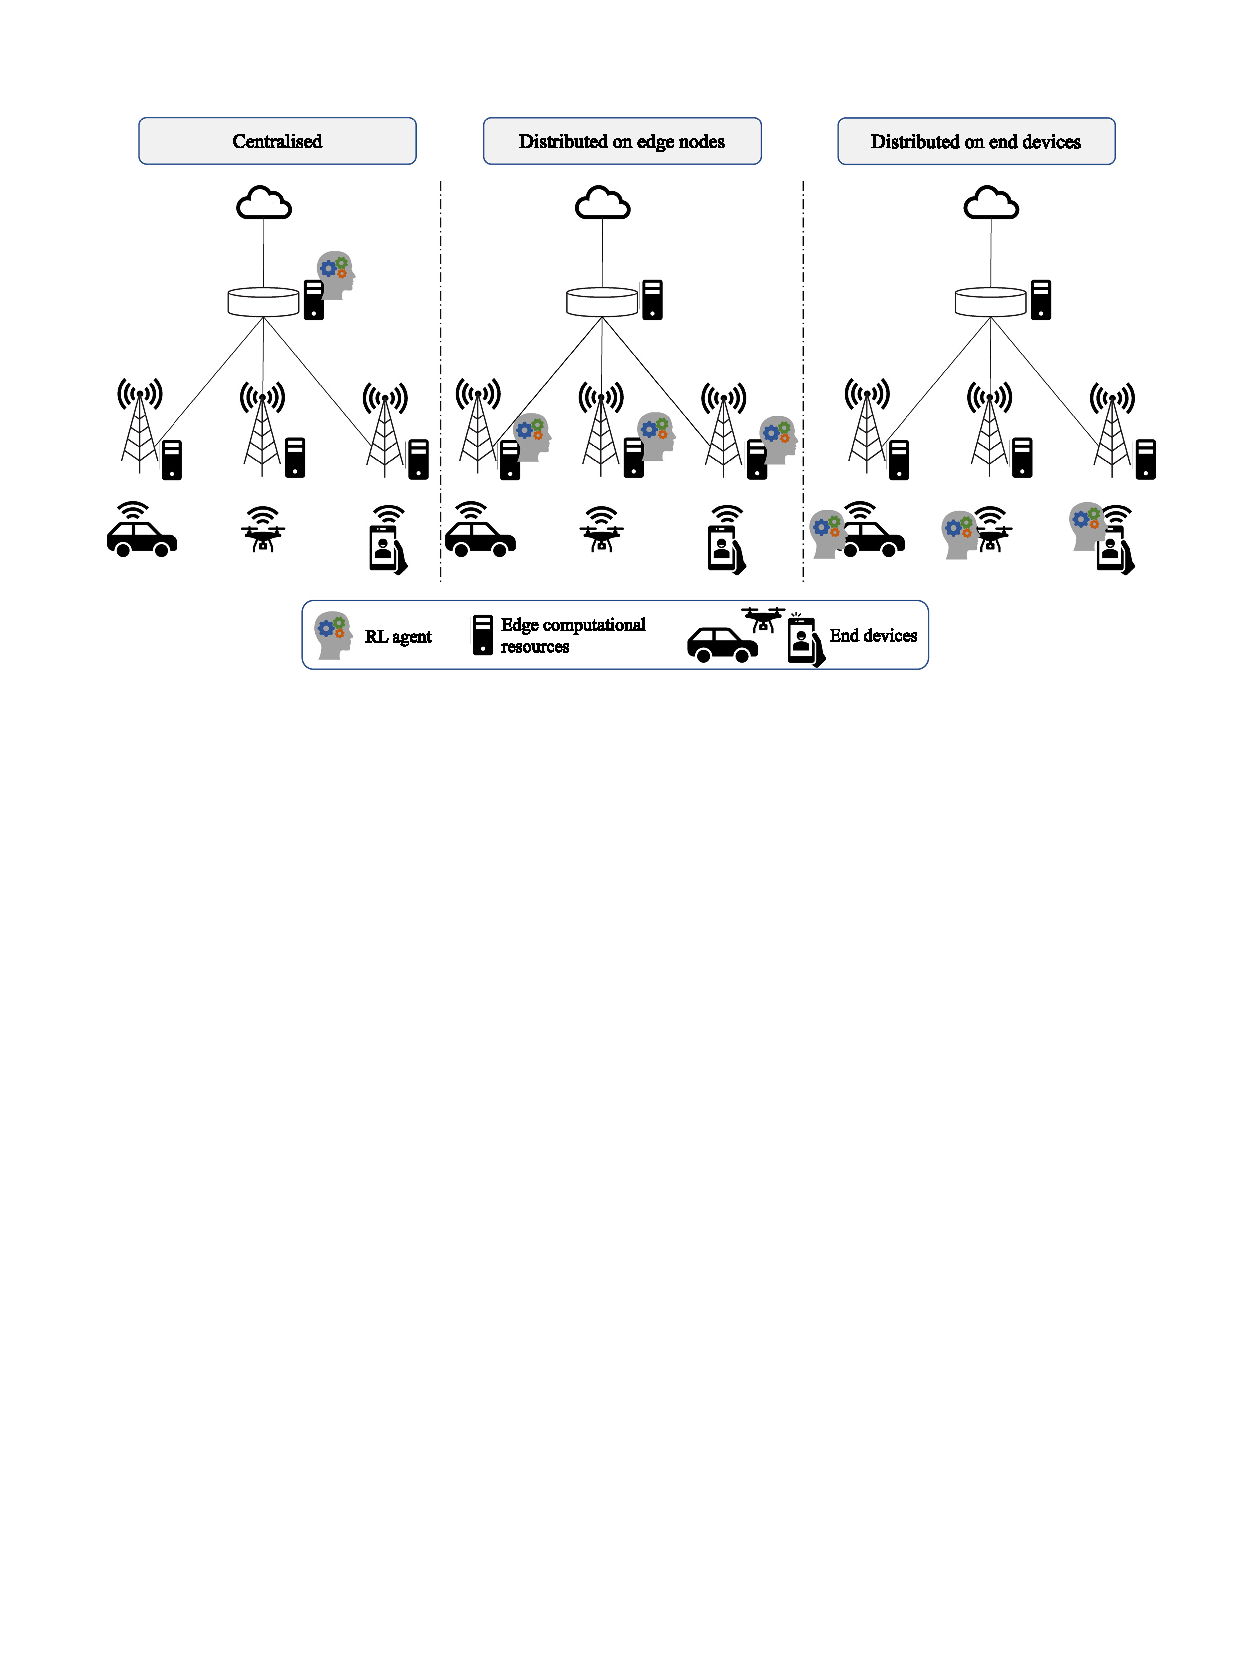
\includegraphics[width=\textwidth]{assets/3/rl_decision_approaches.pdf}
    \caption[Possibili posizionamenti degli agenti RL nella rete edge]{Possibili posizionamenti degli agenti RL nella rete edge. Fonte: \cite{Hortelano2023}}
    \label{fig:2_rl_decision_approaches}
\end{figure}

I lavori analizzati sono stati suddivisi in cinque casi di studio: reti IoT, reti veicolari, reti di UAV\footnote{Aeromobile a pilotaggio remoto (unmanned aerial vehicle), usati come punti di accesso mobili alla rete in caso di disastri naturali o emergenze.}, casi d'uso specifici come realtà virtuale o robotica e studi generici. La maggior parte dei lavori riguarda studi generici, senza focalizzarsi su una rete precisa. Gli algoritmi di RL più utilizzati sono DQN e DDQN, nell'ambito del Q-Learning e quindi value-based. Solo una minima parte dei lavori utilizza PPO. Le principali metriche ottimizzate sono la minimizzazione della latenza e del consumo di energia, solo al terzo posto si trova la massimizzazione dei lavori completati, che in un contesto FaaS può corrispondere al numero di richieste correttamente processate. L'approccio di nostro interesse, cioè distribuito sui nodi edge, risulta essere solo il terzo più comune tra quelli adottati nei lavori analizzati. Anche in questo sondaggio non è presente uno studio all'interno di un contesto di FaaS.

\section{Metodi euristici e RL su ambienti edge}

Tra la moltitudine di lavori incentrati sulla distribuzione del traffico in ambienti edge, abbiamo selezionato quattro lavori di interesse non presenti nei sondaggi citati nella sezione precedente.

In \cite{Chai2021} viene proposto uno schedulatore dinamico basato su priorità e un algoritmo di distribuzione per lavori di priorità diversa. In base alla priorità dei lavori vengono utilizzati approcci diversi: per quelli di alta priorità si impiega un algoritmo euristico basato sul problema dello zaino (knapsack problem), mentre un algoritmo basato sui pesi dei lavori\footnote{Pesi calcolati come la distanza di salti che di un lavoro al lavoro finale, all'interno di un grafo direzionale che rappresenta le dipendenze tra lavori.} e dimensione dei dati è usato per lavori di media priorità.

Sullo stessa tipologia di algoritmi euristici, in \cite{Hsieh2023} viene proposto l'algoritmo Knapsack Potential Game (KPG) per un meccanismo di distribuzione dall'edge al cloud per garantire il servizio per il traffico di alta e bassa priorità. In uno scenario di reti mobili 5G, usando KPG si ottiene un rapporto ottimale di distribuzione per ogni nodo edge che bilancia il costo-efficacia dell'intero sistema, con una bassa complessità computazionale e prestazioni migliori rispetto a due algoritmi base usati come riferimento, uno di tipo greedy e l'altro di tipo cooperativo.

Per metodi strettamente di RL, \cite{Liu2023} si concentra nella minimizzazione del \textit{deadline violation ratio} (DVR), definito come la percentuale di applicazioni non terminate in un orizzonte temporale finito, considerando il carico in ingresso e i ritardi in un contesto di \textit{mobile edge computing} (MEC) in cui la computazione viene portata al bordo della rete cellulare. Viene utilizzato un algoritmo basato su DDPG per determinare la policy ottimale di distribuzione per applicazioni mobile con lavori interconnessi da una rete di dipendenze, ottenendo una riduzione del DVR del 60-70\% rispetto a benchmark esistenti su vari scenari di rete.

Infine in \cite{Zhang2023} viene affrontato il problema per lo stesso contesto MEC 5G, proponendo un algoritmo multi-obiettivo di RL (Multi-Objective Reinforcement Learning, MORL) basato su DDQN per approssimare dinamicamente la decisione ottimale nel contesto di Internet dei veicoli (Internet of vehicles, IoV). MORL generalizza il metodo tradizionale di RL, poiché la ricompensa da un singolo scalare diventa un vettore di scalari. L'agente nell'approccio MORL impara a ottimizzare due o più obiettivi simultaneamente, i quali possono essere correlati positivamente o negativamente (conflittuali) oppure non correlati. MORL può essere pertanto visto come la combinazione dell'ottimizzazione multi-obiettivo con il RL.

L'agente ottiene dall'ambiente definito in \cite{Zhang2023} feedback multipli calcolati in base a parametri di ritardo, energia consumata, carico computazionale ed entropia di riservatezza\footnote{Misura della sicurezza dei dati trasmessi.}. La \Cref{fig:2_morl_vs_rl} mostra la differenza tra MORL e RL tradizionale; notare che l'approccio multi-agente (MARL) è ortogonale a MORL, poiché MARL è caratterizzato dalla presenza di più agenti.

\begin{figure}
    \centering
    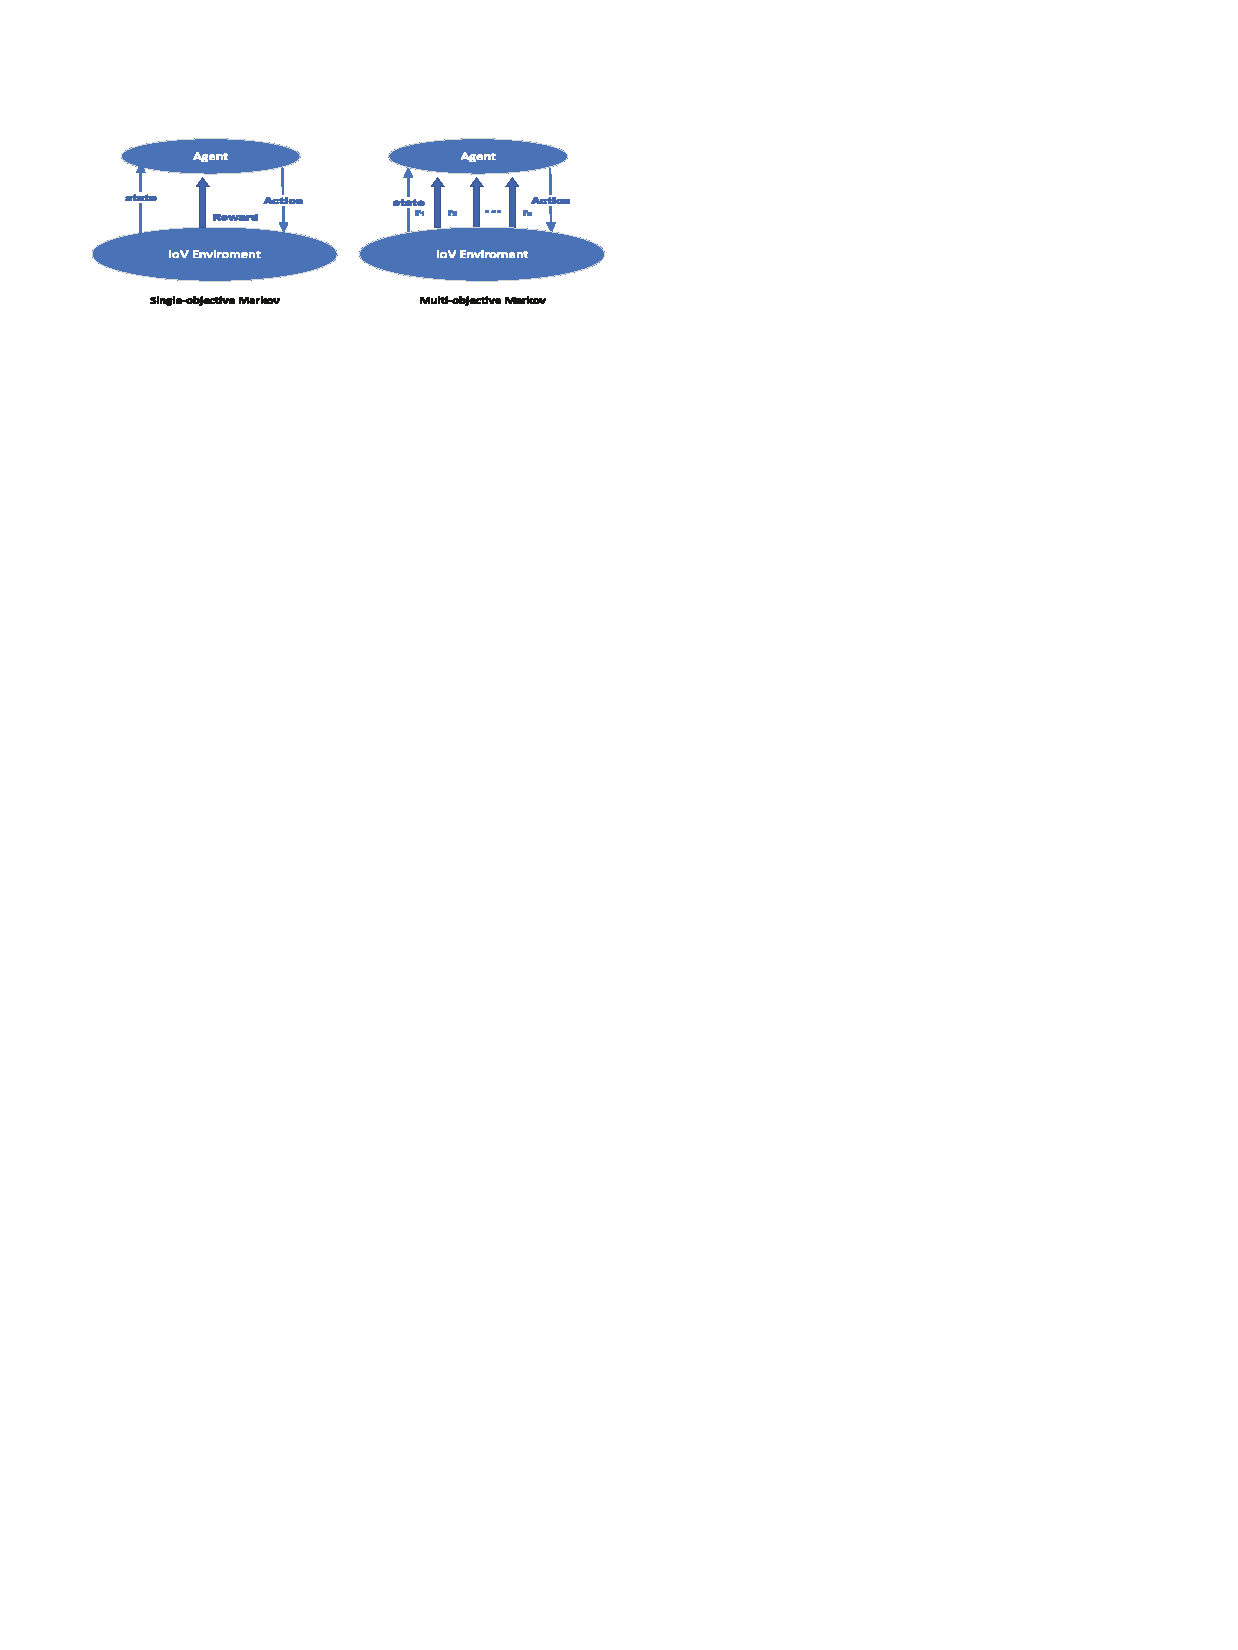
\includegraphics[width=.8\linewidth]{assets/3/morl_vs_rl.pdf}
    \caption[Differenza tra RL tradizionale e RL multi-obiettivo]{Differenza tra RL tradizionale e RL multi-obiettivo. Fonte: \cite{Zhang2023}}
    \label{fig:2_morl_vs_rl}
\end{figure}

\section{Apprendimento per Rinforzo su ambienti FaaS}

Nonostante tutti i lavori menzionati mostrino risultati promettenti utilizzando metodi di RL per affrontare il problema della distribuzione del traffico, nessuno di questi tratta nello specifico sistemi FaaS in ambienti edge, contesto principale di questa tesi.

Considerando unicamente l'ambiente FaaS, \cite{Fuerst2022} propone un algoritmo di bilanciamento del carico progettato per applicazioni FaaS, con l'obiettivo di bilanciare la località, la distribuzione del carico e l'imprevedibilità. I problemi principali con algoritmi di bilanciamento del carico classici è che non considerano le caratteristiche uniche delle funzioni di sistemi FaaS: l'inizializzazione delle funzioni richiede tempo ed è tipicamente omogenea per tutte le tipologie di funzioni, mentre il carico di lavoro è eterogeneo: solo una piccola frazione delle funzioni viene invocata per la maggior parte delle invocazioni. Per questo motivo gli autori utilizzano un sistema di hash coerente\footnote{Tecnica di hash in cui al ridimensionamento della tabella di hash solo una porzione delle chiavi richiede di essere rimappata.} per preservare la località in caso di aggiunta o rimozione di nodi FaaS, fondamentale per gestire i picchi di carico. Sebbene sia simile al lavoro di questa tesi nella gestione di applicazioni serverless, \cite{Fuerst2022} si focalizza su server generici e non considera gli aspetti specifici posti dagli ambienti edge.

In \cite{Petriglia2024}, il lavoro precedente a questa tesi, vengono comparati due algoritmi di RL, PPO e SAC\footnote{Soft Actor-Critic, un algoritmo off-policy con la stessa architettura Actor-Critic di PPO.}, e l'algoritmo generico NEAT\footnote{NeuroEvolution of Augmenting Topologies, che si basa sulla generazione evolutiva di reti neurali.} addestrando un singolo agente in un ambiente che modella la distribuzione del carico in un sistema di computazione edge-FaaS. Il sistema modellato è raffigurato in \Cref{fig:2_single_agent_env} e coinvolge un nodo in grado di processare le richieste localmente, inoltrarle ai nodi vicini e rifiutarle. Gli algoritmi sono stati provati su tre tipologie di carico. L'agente, nel sistema proposto, osserva la disponibilità di inoltro e il carico in ingresso al passo successivo. PPO è risultato l'algoritmo migliore rispetto a SAC e NEAT in termini di richieste rifiutate per episodio.

Il lavoro di questa tesi è un diretto proseguimento di \cite{Petriglia2024}: si supera l'ambiente a singolo agente introducendo un ambiente multi-agente (descritto nel \Cref{sec:4_modellazione}), per addestrare gli agenti viene utilizzato PPO in due configurazioni MARL, le tre tipologie di carico di prova sono riproposte, tuttavia una di questa viene sostituita con dati reali e non generati (descritta nella \Cref{sec:5_scenario_reale}).

\begin{figure}
    \centering
    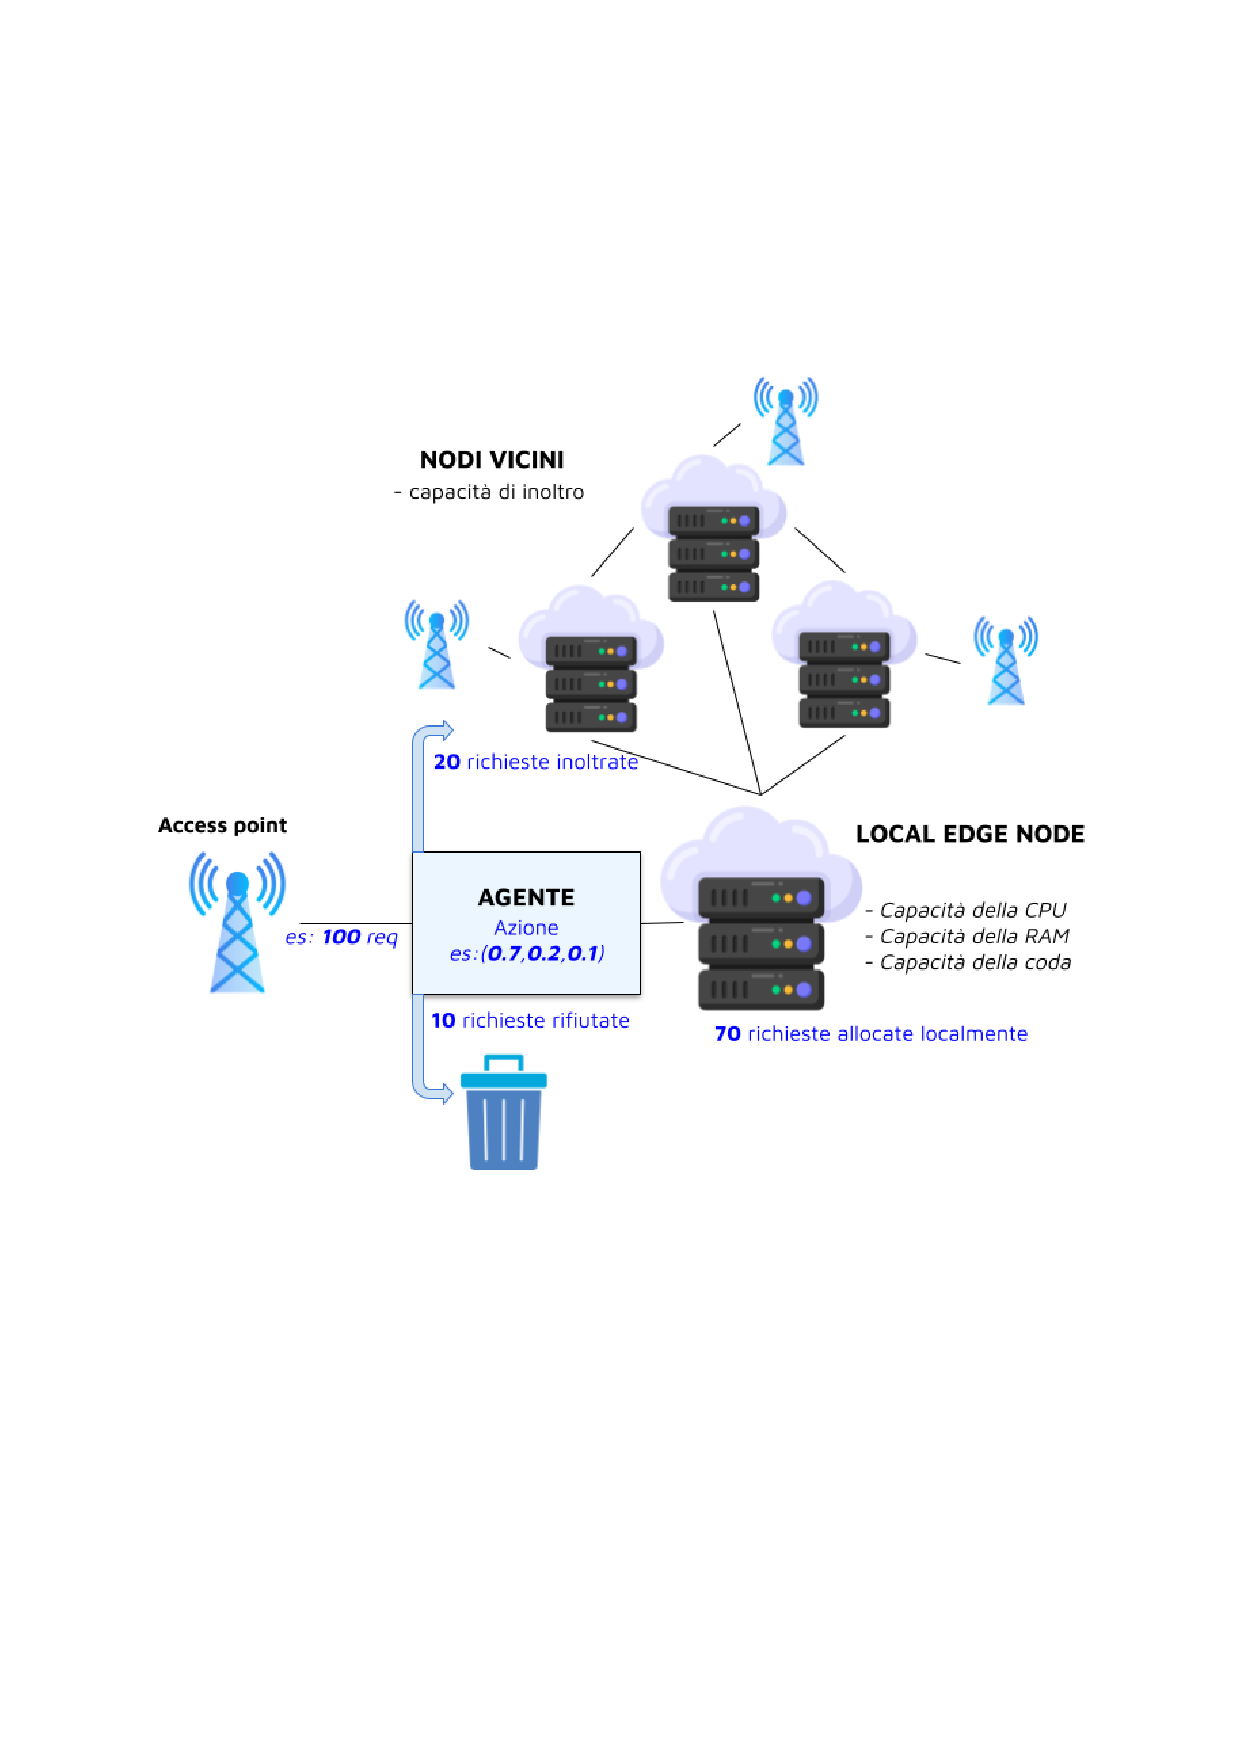
\includegraphics[width=.8\linewidth]{assets/3/single_agent_env.pdf}
    \caption[Sistema modellato a singolo agente.]{Sistema modellato a singolo agente. L'agente decide come distribuire le richieste attraverso una distribuzione, nell'esempio $(0.7, 0.2, 0.1)$, che viene poi convertita nel numero di richieste da distribuire $(70, 20, 10)$. Fonte: \cite{Petriglia2024}}
    \label{fig:2_single_agent_env}
\end{figure}